\documentclass[conference]{IEEEtran}
\IEEEoverridecommandlockouts
% The preceding line is only needed to identify funding in the first footnote. If that is unneeded, please comment it out.
\usepackage{cite}
\usepackage{amsmath,amssymb,amsfonts}
\usepackage{algorithmic}
\usepackage{graphicx}
\usepackage{textcomp}
\usepackage{xcolor}
\usepackage{graphicx}
\usepackage{lipsum}
\usepackage{booktabs} 
\usepackage{caption}
\usepackage[linesnumbered,ruled,vlined]{algorithm2e}
\def\BibTeX{{\rm B\kern-.05em{\sc i\kern-.025em b}\kern-.08em
    T\kern-.1667em\lower.7ex\hbox{E}\kern-.125emX}}
\begin{document}

\title{Joint Optimization of IRS-Aided MIMO VLC System Capacity Based on DRL\\
}

\author{\IEEEauthorblockN{Shengchen Zhang, Sirui Deng, Jiahe Zhang, Xizuho Zhang, Haowei Qin, Linqiong Jia}
\IEEEauthorblockA{\textit{The School of Electronic and Optical Engineering,Nanjing University of Science and Technology,} \\
Nanjing, 210094, China\\
Shengchen.Zhang@njust.edu.cn, qinqinhw@njust.edu.cn, jialinqiong@njust.edu.cn}
~\\
}

\maketitle

\begin{abstract}
As an emerging technology, intelligent reflecting surface (IRS) can significantly 
improve the performance of visible light communication (VLC) by 
digitally adjusting the reflection parameters. In this paper, we consider improving 
VLC performance by deploying IRS in a multiple-inputs multiple-output (MIMO) environment. 
Firstly, we established the pairing relationship between IRS, light emitting diode (LED) 
and receiving photodiode (PD) and gave them constraints. Then we introduced the reflection coefficient 
vector of IRS and the power allocation vector of LED. Finally, through the deep 
reinforcement learning (DRL), we propose a 
twin delayed deep deterministic policy gradient (TD3) algorithm based on markov decision 
process (MDP) to solve the optimization problem of maximizing the capacity. Moreover, 
we have compared deep deterministic policy gradient (DDPG) algorithm to TD3. The last numerical 
results show the convergence, stability and effectiveness of the TD3 algorithm.
\end{abstract}
\section{Introduction}
   With the rapid development of wireless communication technology, there is a growing
   demand for ultra-large capacity in communication systems. To satisfy this demand, 
   the communication system not only widely adopts various technologies to improve 
   the spectral efficiency of radio frequency (RF) communication, such as large-scale 
   multiple-inputs multiple-output (MIMO) and non-orthogonal multiple access (NOMA), 
   but also builds a new physical layer architecture which include visible light, 
   millimeter wave (mmWave) and terahertz (THz) frequency as an improvement and 
   supplementation for RF communication\cite{1}.

 The pace of optical wireless communication (OWC) has been 
 very fast that visible light communication (VLC) which based on using prevalent 
 light emitting diode (LED) lighting devices has been a valuable OWC technology. 
 While existing wireless technologies are depleting the 
 electromagnetic (EM) spectrum available in RF bands, VLC utilizes unregulated, 
 undeveloped, and large EM bands in the visible range, which means that VLC has 
 the advantage of being free of spectrum licensing. VLC also has many favorable 
 benefits, such as broad bandwidth, less 
 interference with RF communications, excellent ability for reusing 
 high frequency\cite{3} and higher power efficiency\cite{4}. Meanwhile, MIMO
  technology has been considered to achieve high data rates and 
     \begin{figure}[htbp]
     \scalebox{0.34}{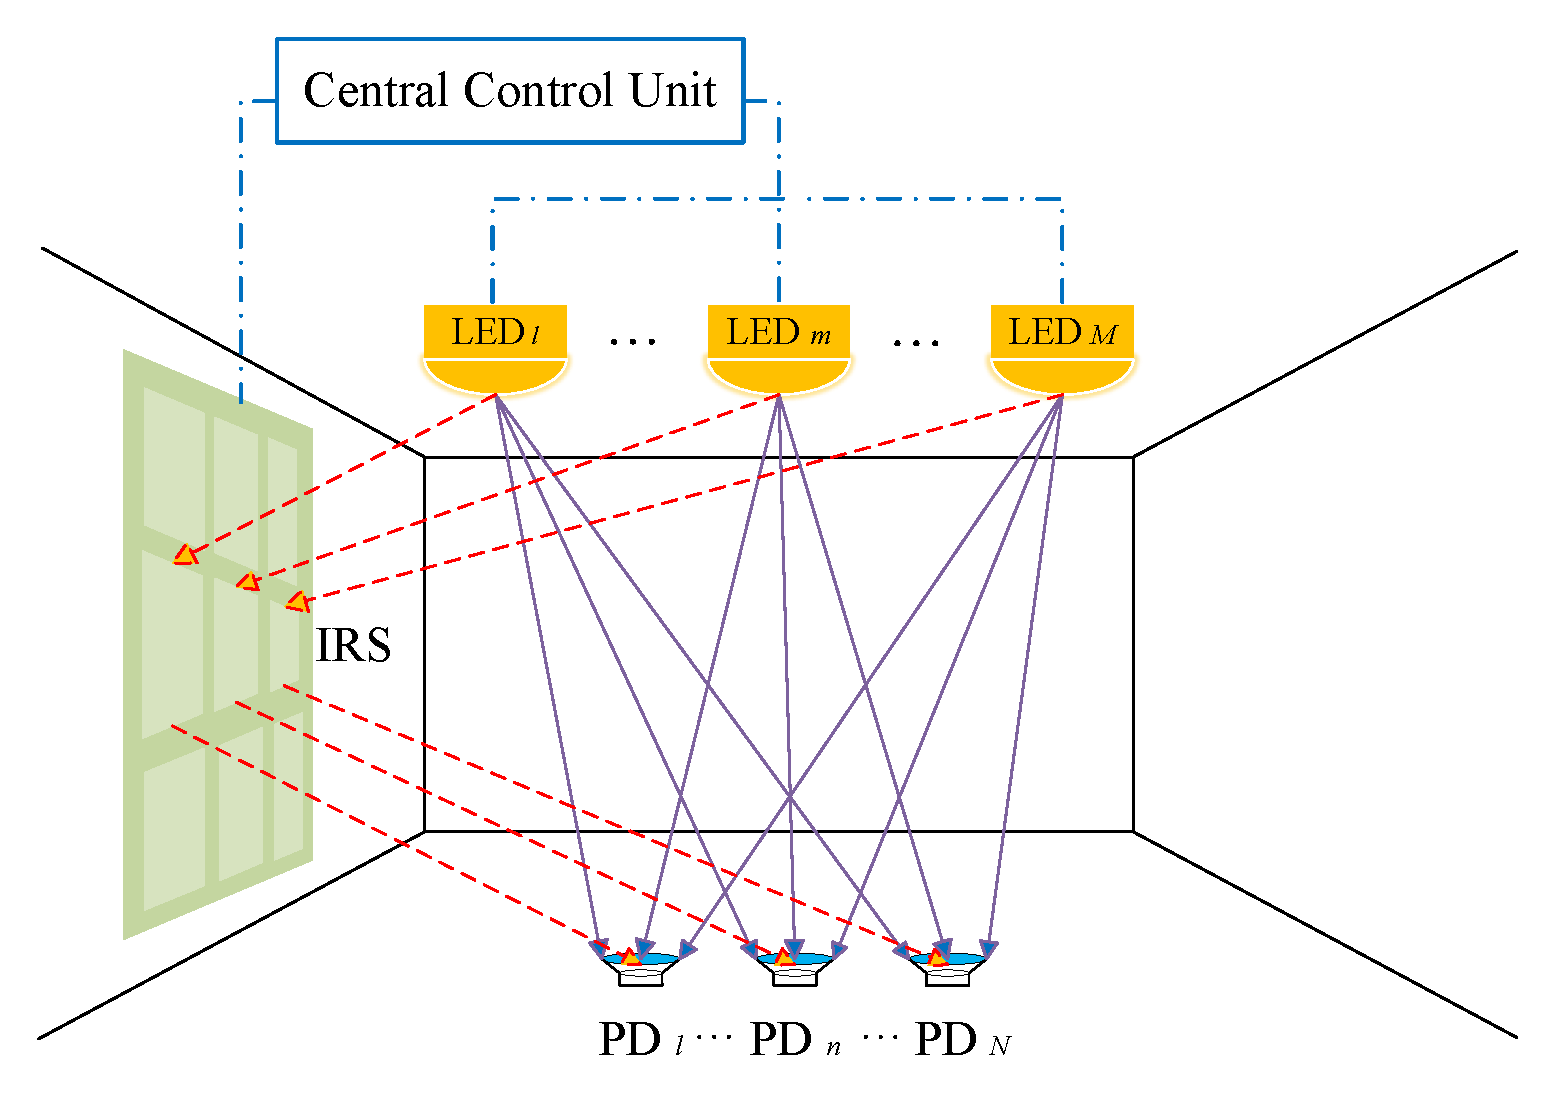
\includegraphics{Space modle.pdf}}
     \caption{ Tunable IRS-Aided MIMO VLC System.}
     \label{fig:1}
    \end{figure}
 reliability without consuming additional time and spectrum resources of 
 VLC system\cite{5}\cite{6}. But visible light channels normally follow the typical 
 Lambertian model, so that the channel gain depends on the position of the 
 transceiver. When the receiving photodiode (PD) distance 
 is close, the MIMO channels have a serious correlation and the channel matrix 
 condition number is too large to obtain the ideal multiplexing gain\cite{7}.
 To increase the channel capacity, the correlation 
 of MIMO VLC channels is detailed by singular value decomposition (SVD) of the 
 signal of $4 \times 4$ MIMO VLC system, and the system performance 
 is improved by adaptive power and bits allocation strategy \cite{9}. 

 Since the VLC system mainly depends on the 
 line of sight (LoS), and the signal gain of non-line of sight (NLoS) is 
 negligible, the communication link will be interrupted and the  
 situation will be affected once the LoS link is blocked. Nowdays, the emerging 
 intelligent reflecting surface (IRS) start owning the capability of reconfiguring 
 the wireless electromagnetic environment. Optical IRS overcomes the above 
 shortcomings by providing NLoS optical signal transmission paths. 
 Through controlling the relevant parameters of 
 the IRS, the VLC system can surmount the high dependence of LoS, enhance 
 the received signal power,expand the communication range and relax the 
 dimming constraints on the basis of meeting the lighting needs of users\cite{7}. 

  Recently, with the development of optical 
  metasurface technology\cite{12}, the sensitivity and response speed of the IRS to 
  visible light have been improved quickly and steadily\cite{13}\cite{14}. An innovative 
  IRS element with adjustable phase and amplitude is proposed, which also has 
  the function of reflected signal power control\cite{15}. Deep-Q-learning 
  is used to optimize
  resource management and maximize the spectral efficiency\cite{16}.

  We aims at optimizing the pairing matrix for the 
  IRS and maximizing the capacity of IRS-aided MIMO VCL system. And in this 
  system, the reflection coefficient is adjustable and 
  waiting to be optimized. In paper\cite{17}, it modeled IRS-reflected channel 
  and characterize the IRS-aided MIMO VLC capacity under different transmitter 
  emission power constraints. We will use the capacity of the system as a 
  maximization function. The main contributions in 
  our work are summarized as follows:
     \begin{itemize}
     \item First, we established a model of IRS-aided MIMO VCL system as 
     shown in Fig.1. Based on the above, we constructed a general channel 
     model between the signal transmitter and receiver, 
     and it also follows the corresponding dimming 
     power constraints and pairing relationships between the LED, IRS and PD.
     \item Next, we put forward an optimization issues which aims at maximize 
     system capacity characterized in\cite{17}. Because the 
     parameters to be optimized include the reflection coefficient of the 
     IRS, the LED power constraint, and the pairing relationship 
     between the IRS, LED and PD, which is a non-convex mixed 
     integer optimization problem, it is difficult to solve  
     directly. Therefore, we established a markov decision 
     process (MDP), and use twin delayed deep deterministic policy gradient (TD3) 
     algorithm to find the optimal solution when the capacity is 
     maximum.
     \item The final results show that the algorithm based on TD3
      are effective and convergent, meaning that the 
     calculational complexity is substantially decreased and more efficient 
     and equitable resource allocation scheme can be solved for IRS-aided VLC system.
     \end{itemize}

   The rest of this article consists of the following. In Section II, a 
   spatial system and channel model is constructed, and in Section III 
   we proposed a TD3 algorithm based on deep 
   reinforcement learning (DRL) to solve the optimal solution. 
   Section IV provides numerical results 
   to evaluate the performance of the proposed algorithm in IRS-aided 
   MIMO VLC system. In the end, Section V summarizes the article.
     \begin{figure}[htbp]
     \scalebox{0.62}{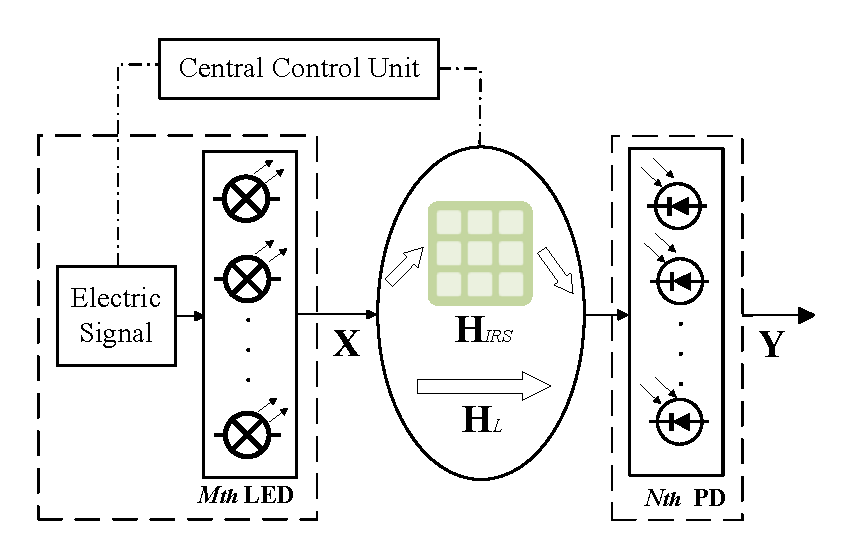
\includegraphics{Theoretical model.pdf}}
     \caption{IRS-Aided MIMO VLC System Model.}
     \label{fig:2}
     \end{figure}

\section{MODEL AND PROBLEM FORMULATION}

 \subsection{System Model}
   Consider an IRS-aided MIMO VLC system spatial model as shown in 
   Fig.~\ref{fig:1}.
   There are $M$ LEDs, $N$ PDs, and $K$ IRS elements in 
   the system. By changing the reflection coefficient of the IRS element, 
   the spatial freedom degree of the MIMO system can be improved, 
   and the capacity can be further improved. That is, 
   the IRS-aided MIMO VLC system can change the channel matrix 
   and reduce the correlation of the MIMO channel through 
   changing the IRS reflection.
 \subsection{Channel Model}
   Consider an $M \times N$ dimensional IRS-aided MIMO VLC system as shown 
   in Fig.~\ref{fig:2}. The reflection coefficients of $K$ IRS 
   elements in the system are represented by the vector 
   ${\bf{r}} = ({r_1}, \cdots , {r_K})$, $0 \le {r_k} \le \alpha $,  
   and the ${r_k}$ represents the maximum value of the reflection coefficient. 
   When the $k$-th IRS element is operating, the central 
   control unit controls the intensity of the reflected light from 
   the IRS elements by setting the ${r_k}$.
   
   The vector of the transmitted signal of $M$ LEDs can be 
   represented by ${\bf{X}} = {({X_1},{X_2}, \cdots ,{X_M})^T}$. 
   There are $N$ PDs receiving signals at the same 
   time. The received signal vector is ${\bf{Y}} = {({Y_1}, \cdots ,{Y_N})^T}$, 
   and it has the following relationship with ${\bf{X}}$:
      \begin{table*}
      \centering
      \caption*{}
      \begin{tabular*}{\textwidth}{@{\extracolsep{\fill}} c}
      \textbf{ \begin{minipage}{1\textwidth}
      \begin{equation}
      h_{n,k,m}^{\rm{(IRS)}} = \left\{ \begin{array}{l}
      \dfrac{{(\kappa  + 1){A_{{\rm{PD}}}}{{\cos }^\kappa }(\phi _{m,k}^{{\rm{LR}}})\cos (\psi _{k,n}^{{\rm{RD}}})\cos (\theta _{k,n}^{{\rm{RD}}})}}{{2\pi {{\left( {{d_{kn}} + {d_{km}}} \right)}^2}
      {{{\rm{(}}{\overrightarrow{\rm N}}{_k^{{\rm{IRS}}}}{\rm{)}}^T}}
      {\overrightarrow{\rm E}}{_{k,n}^{{\rm{RD}}}}}}{T_s}(\psi _{k,n}^{{\rm{RD}}})g(\psi _{k,n}^{{\rm{RD}}}),0 < \psi _{k,n}^{{\rm{RD}}} < {\Psi _C}\\
      \\ 0,{\kern 231pt} \psi _{k,n}^{{\rm{RD}}} > {\Psi _C}
      \end{array} 
      \right.
      \tag{5}
      \label{eq5}
      \end{equation}
      \end{minipage}
      }\\\\
      \bottomrule
      \end{tabular*}
      \end{table*}

     \begin{equation}
     \bf{Y} = \bf{HX} + \bf{Z} \label{eq1}
     \end{equation}
   where ${\bf{Z}} = {({Z_1}, \cdots ,{Z_N})^T}$ is an additive gaussian white noise 
   vector, namely ${\bf{Z}}\sim {\cal N}({\bf{0}},{\sigma ^2}{{\bf{I}}_N})$.

   In the presence of IRS, the channel matrix includes the direct path gain ${{\bf{H}}_L}$ of 
   LEDs and the reflected path gain ${{\bf{H}}_{IRS}}$ of IRS elements. Thus, the channel 
   matrix can be expressed as ${\bf{H}} = \left[ {{{\bf{H}}_{\rm{L}}} + {{\bf{H}}_{{\rm{IRS}}}}} \right]$, 
   ${\bf{H}} \in {\mathbb{R} ^{N \times M}}$.
   The gain of direct path can be expressed as
     \begin{equation}
     {{\bf{H}}_{\rm{L}}} = {\left[ {h_{nm}^{(L)}} \right]_{N \times M}} \label{eq2}
     \end{equation}
   where $h_{nm}^{(L)}$ represents the LoS channel gains from the $m$-th LED to 
   $n$-th PD, which can be calculated from the relative position between the 
   PD and LED:
\begin{equation}
h_{nm}^{({\rm{L}})} = \left\{ 
 \begin{array}{l}\!\!\!
\dfrac{{(\kappa  + 1){A_{{\rm{PD}}}}}}{{2\pi d_{nm}^2}}{\cos ^\kappa }({\phi _{n,m}})g({\psi _{n,m}})T({\psi _{n,m}})\cos ({\psi _{n,m}}),
 \\ {\kern 116pt} 0 < {\psi _{n,m}} < {\Psi _C}
 \\ \\ 0,{\rm{                                      }}
 {\kern 125pt} {\rm{   }}{\psi _{n,m}} > {\Psi _C}
 \end{array} \right.\
\label{eq3}
\end{equation}
   where ${A_{{\rm{PD}}}}$ is the detection area of the receiving PD, 
   $\kappa  =  - 1/{\log _2}(\cos {\Phi _{1/2}})$ is the Lambertian 
   radiation order of the LED, the ${\Phi _{1/2}}$ is 
   the half-radiation angle of the light source, ${d_{nm}}$ represents 
   the distance between the LED and PD, ${\phi _{n,m}}$ is the radiation 
   angle from the $m$-th LED to $n$-th PD, 
   ${\psi _{n,m}}$ is the angle of incidence from $m$-th LED to $n$-th PD, 
   ${\Psi _C}$ is the 
   half-field of view of the PD, $g({\psi _{n,m}})$ is the gain of the 
   optical filter. The $T({\psi _{n,m}})$ is the gain of the optical 
   concentrator, which can be calculated by the following formula:     
     \begin{equation}
     T({\psi _{n,m}}) = \left\{ \begin{array}{l}
     \dfrac{{n_r^2}}{{{{\sin }^2}{\Psi _C}}},0 < {\psi _{n,m}} < {\Psi _C}\\
     \\ 0,{\kern 47pt} 
      {\psi _{n,m}} > {\Psi _C}
     \end{array} \right.
     \label{eq4}
     \end{equation}
   where  $n_r$ denotes the refractive index of the optical concentrator.

   Regardless of the effect of the reflection coefficient, the channel gain 
   reflected by the $k$-th IRS element from the $m$-th LED to  
   $n$-th PD is expressed in $h_{n,k,m}^{}$ and can be calculated by the 
   Eq.(\Ref{eq5}) at the top of this page. In Eq.(\Ref{eq5}),
    ${d_{kn}}$ and ${d_{km}}$ respectively represent the distance from the 
   $k$-th IRS element to the $n$-th PD and the $m$-th LED light source, 
   $\phi _{m,k}^{{\rm{LR}}}$ represent the radiation angle from the $m$-th LED 
   light source to $k$-th IRS element, the $\theta _{k,n}^{{\rm{RD}}}$ 
   represents the radiation angle from the $k$-th IRS element to $n$-th 
   PD, $\psi _{k,n}^{{\rm{RD}}}$ represents the angle of incidence 
   from the $k$-th IRS element to $n$-th PD, 
   ${T_s}(\psi _{k,n}^{{\rm{RD}}})$ and $g(\psi _{k,n}^{{\rm{RD}}})$ 
   still represent the optical concentrator gain and optical filter gain of PD, 
   ${\overrightarrow{\rm N}}{_k^{{\rm{IRS}}}}$ represents 
   the unit normal vector of the $k$-th reflector surface and 
   ${(}{\overrightarrow{\rm N}}{_k^{{\rm{IRS}}}}{{\rm{)}}^T}$
   represents the rank of the vector, 
   ${\overrightarrow{\rm E}}{_{k,n}^{{\rm{RD}}}}$
   represents the directional unit vector from the $k$-th IRS element 
   to the $n$-th PD.
   ${{\bf{H}}_{\rm{IRS}}}$ can be represented in terms of binary matrices 
   ${\bf{G}} = [{{\bf{g}}_1}, \cdots ,{{\bf{g}}_M}] \in {\{ 0,1\} ^{K \times M}}$
   and ${\bf{F}} = [{{\bf{f}}_1}, \cdots ,{{\bf{f}}_N}] \in {\{ 0,1\} ^{K \times N}}$,
   where ${\bf{G}}$ is the pairing between the IRS elements and the LEDs, 
   ${\bf{F}}$ is the pairing between the
   IRS elements and the PD. Since the beam width of the reflected light of the 
   IRS elements is highly spatially limited, there is no crosstalk between the 
   IRS reflection channels and each IRS element can only provide a reflection 
   link for a pair of LED and PD. The binary matrix 
   ${\bf{G}} \in {\{ 0,1\} ^{K \times M}}$ can be expressed as
     \begin{equation}
     {\bf{G}}= [{{\bf{g}}_1}, \cdots ,{{\bf{g}}_M}] =
     \left[ {\begin{array}{*{20}{c}}
     {{g_{1,1}}}& \cdots &{{g_{1,M}}}\\
     \vdots & \ddots & \vdots \\
     {{g_{K,1}}}& \cdots &{{g_{K,M}}}
     \end{array}} \right] = {[{{\bf{\tilde g}}_1}, \cdots ,{{\bf{\tilde g}}_K}]^T}
     \tag{6}\label{6}
     \end{equation}
   where ${g_{k,m}} = 1$ indicates that the $k$-th IRS element reflects the 
   VLC signal emitted by $m$-th LED, and ${{\bf{g}}_m}$ and 
   ${{\bf{\tilde g}}_k}$ respectively represent the $m$-th column
   and $k$-th row of ${\bf{G}}$.
   The binary matrix 
   ${\bf{F}} \in {\{ 0,1\} ^{K \times N}}$ is used to 
   represent the pairing between the IRS elements and PDs, 
   which can be expressed as
     \begin{equation}
     {\bf{F}} = [{{\bf{f}}_1}, \cdots ,{{\bf{f}}_N}] = \left[ {\begin{array}{*{20}{c}}
     {{f_{1,1}}}& \cdots &{{f_{1,N}}}\\
     \vdots & \ddots & \vdots \\
     {{f_{K,1}}}& \cdots &{{f_{K,N}}}
     \end{array}} \right]
     \tag{7}\label{eq7}
     \end{equation}
   where ${f_{k,n}} = 1$ means that the reflected light of the $k$-th IRS 
   element is received by $n$-th PD, and ${{\bf{f}}_n}$ means 
   that the $n$-th PD 
   receives the VLC signal reflected by the IRS element. 
   When ${g_{k,m}} = 1$ and ${f_{k,n}} = 1$, the $k$-th IRS elements reflects 
   the signal from the $m$-th LED to $n$-th PD. 
   When considering the reflection 
   coefficient of the IRS elements, the channel gain 
   ${{\bf{H}}_{\rm{IRS}}} \in {\mathbb{R} ^{N \times M}}$ through the reflection 
   paths can be expressed as
     \begin{equation}
     {{\bf{H}}_{\rm{IRS}}} = {\left[ {{{\left( {{{\bf{f}}_n} \odot {{\bf{g}}_m}} \right)}^T}\left( {{{\bf{r}}^T} \odot {{\bf{h}}_{n,m}}} \right)} \right]_{N \times M}}
     \tag{8}\label{8}
     \end{equation}
   where ${{\bf{h}}_{n,m}} = {\left[ {h_{n,1,m}^{\rm{(IRS)}}, \cdots ,h_{n,K,m}^{\rm{(IRS)}}} \right]^T}$ 
   represents the gain of the reflection path of $K$ IRS elements between 
   the $m$-th LED and the $n$-th PD without considering the reflection 
   coefficient of IRS elements. $ \odot $ denotes the Hadamard product. 
   Therefore, we can define the channel matrix
   ${\bf{H}} = \left[ {{{\bf{H}}_{\rm{L}}} + {{\bf{H}}_{{\rm{IRS}}}}} \right] = {\left[ {h_{n,m}^{total}} \right]_{N \times M}}$ 
   ,which the ${h_{n,m}^{total}}$ can be expressed as
     \begin{equation}
     h_{n,m}^{total} = h_{n,m}^{(L)} + {\left( {{{\bf{f}}_n} \odot {{\bf{g}}_m}} \right)^T}\left( {{{\bf{r}}^T} \odot {{\bf{h}}_{n,m}}} \right)
     \tag{9}\label{9}
     \end{equation}

   Since each IRS element can only provide reflections for a pair of LED and PD, 
   ${g_{k,m}}$ and ${f_{k,n}}$ need to meet the constraints:
     \begin{equation}
     \sum\nolimits_{m = 1}^M {{g_{k,m}}}  \le 1,\forall k \in {\cal K}
     \tag{10}\label{10}
     \end{equation}
     \begin{equation}
     \sum\nolimits_{n = 1}^N {{f_{k,n}}}  \le 1,\forall k \in K
     \tag{11}\label{11}
     \end{equation}
\begin{figure*}[htbp]
%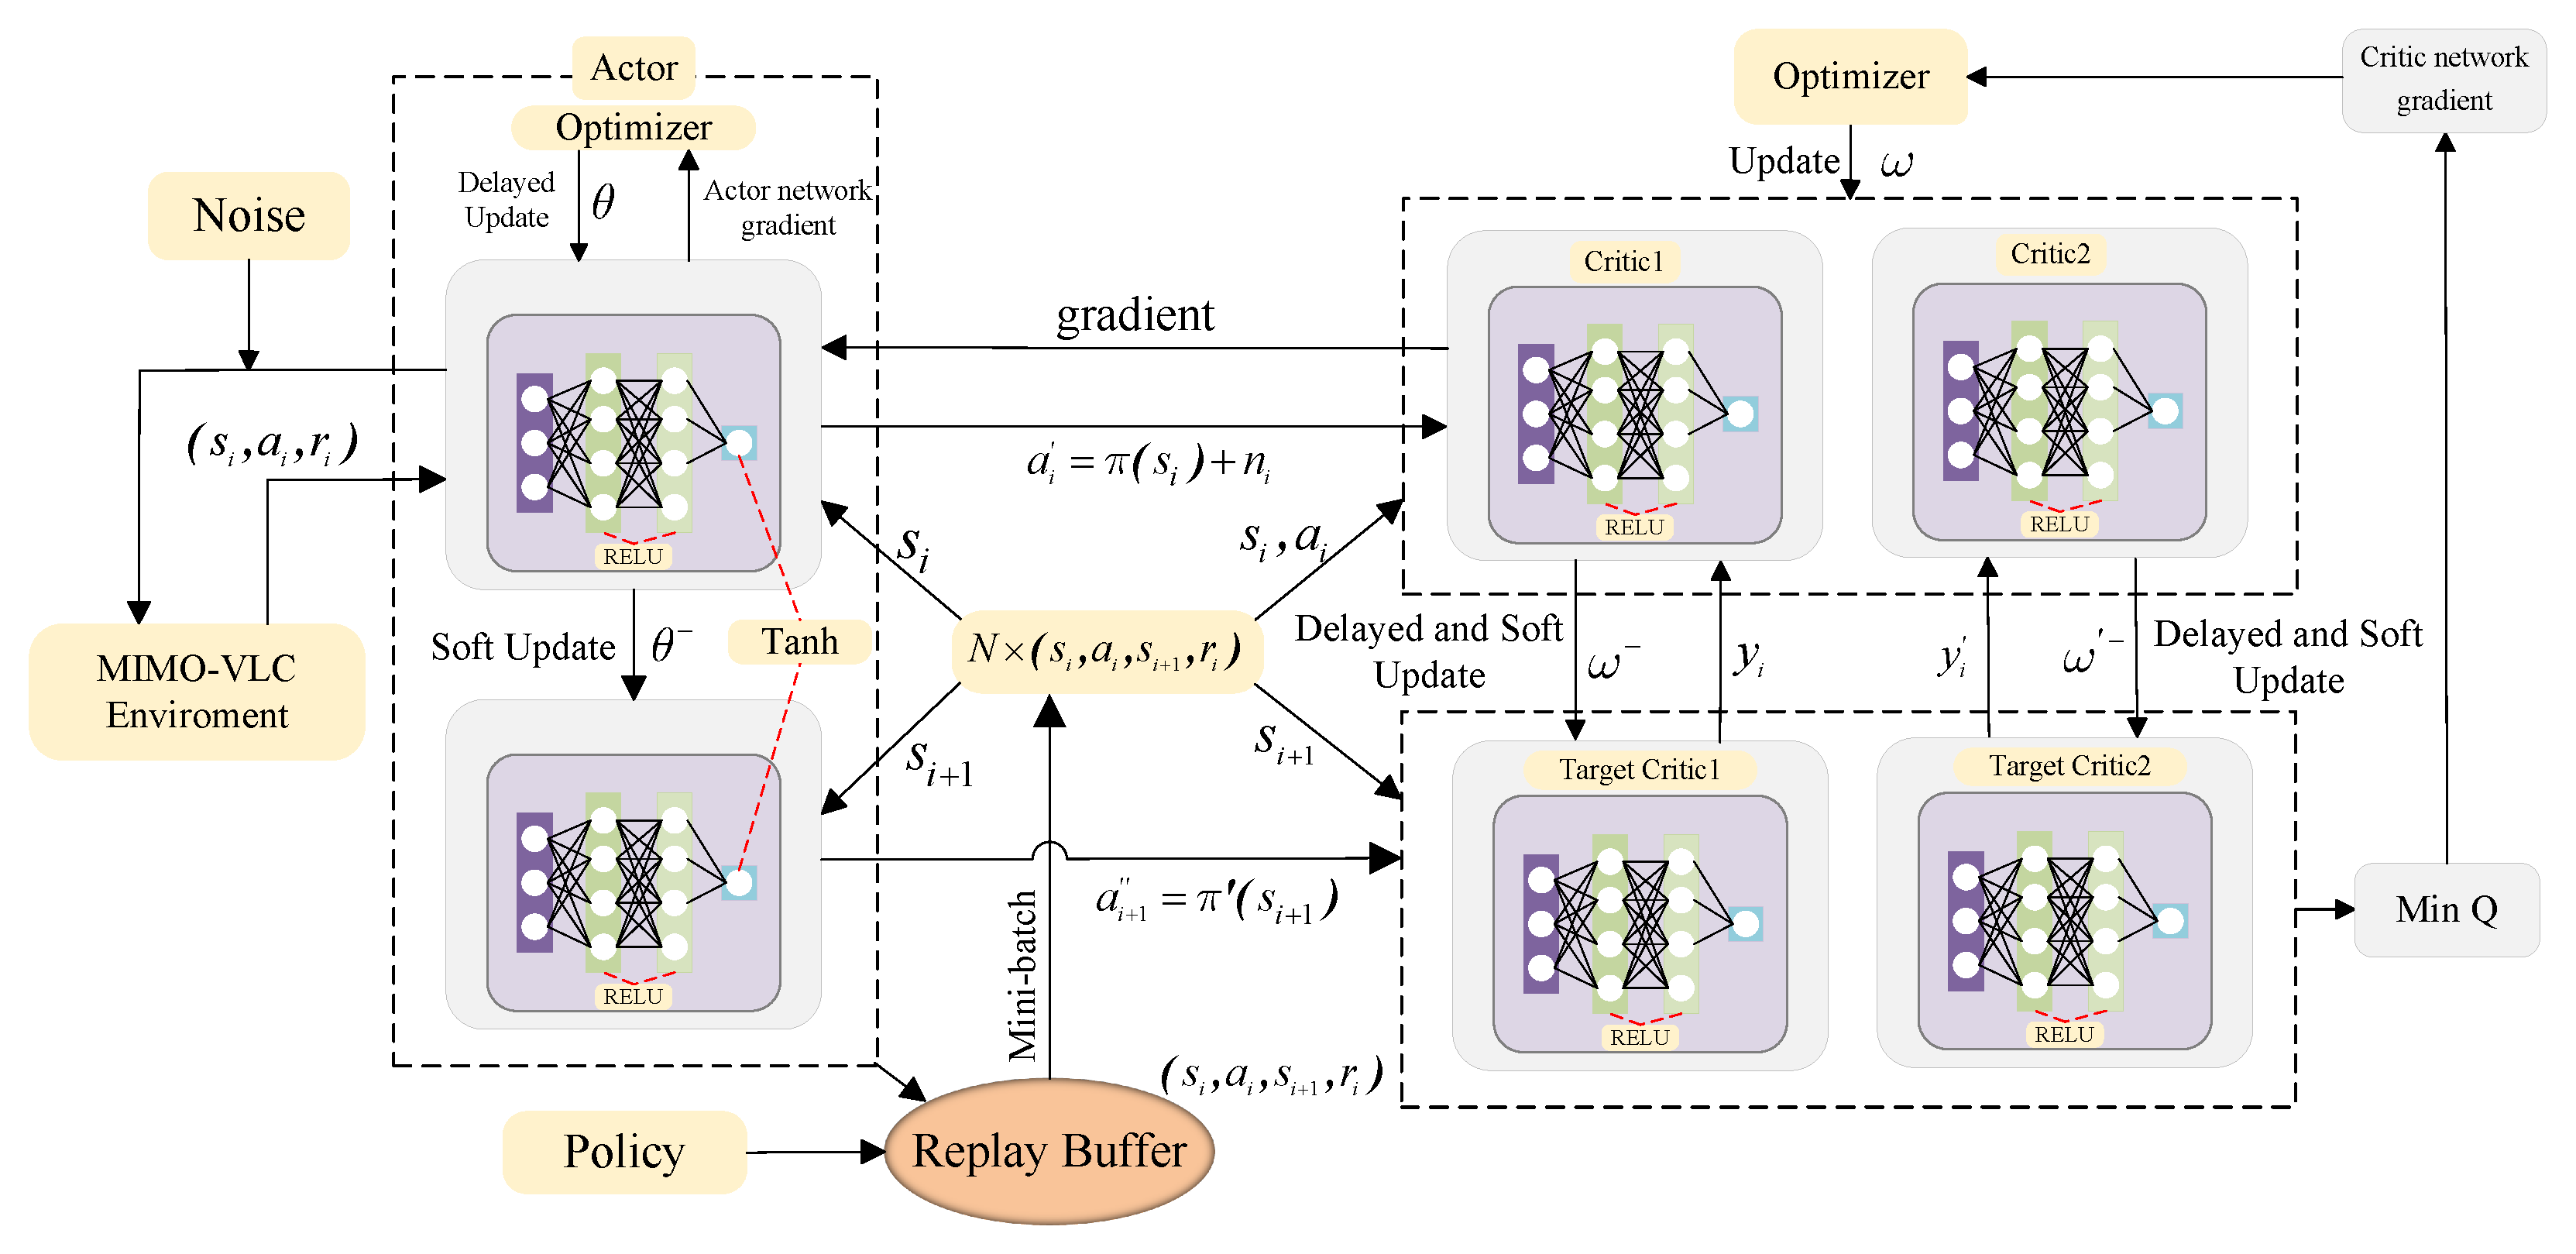
\includegraphics[width=3.33in, keepaspectratio]{TD3 principle.pdf}
\scalebox{0.32}{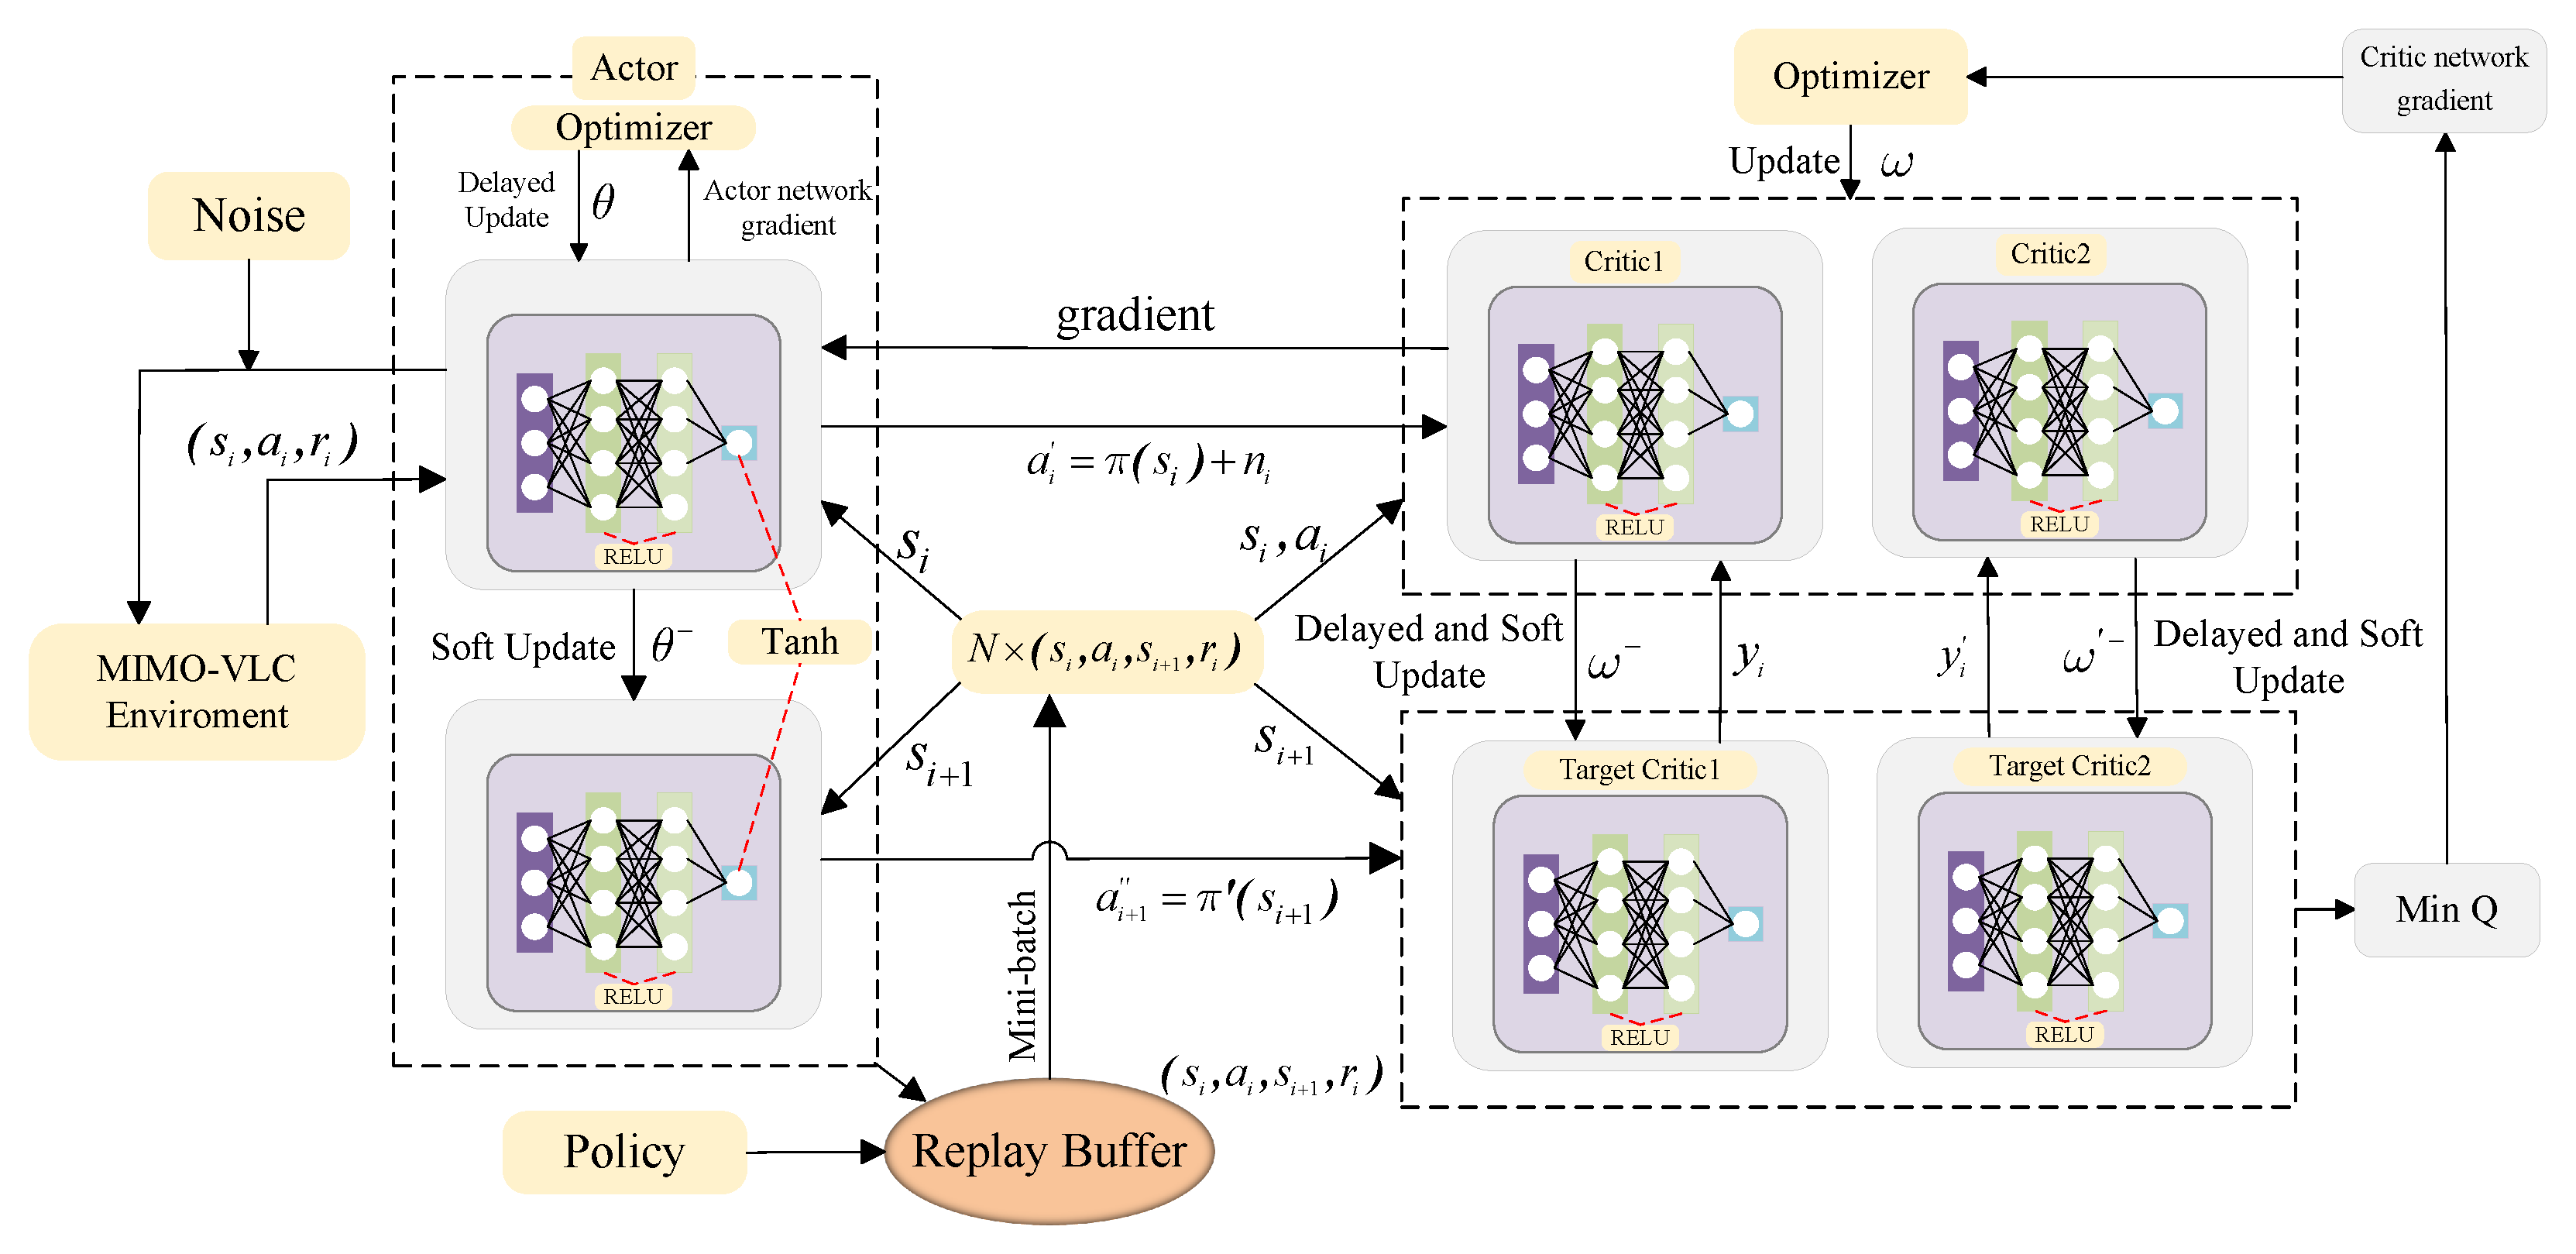
\includegraphics{TD3 principle.pdf}}
\caption{TD3 prinpicle}
\label{fig:3}
\end{figure*}
   In addition, the emitted light intensity of the LED  
   needs to meet the peak power constraint and the dimming constraint:
     \begin{equation}
     0 \le {X_m} \le {A_m},{\kern 1pt} {\kern 1pt} {\kern 1pt} {\kern 1pt} {\kern 1pt} {\kern 1pt} {\kern 1pt} {\kern 1pt} {\kern 1pt}   m = 1, \cdots ,M
      \tag{12}\label{12}
     \end{equation}
     \begin{equation}
      E\left[ {{X_m}} \right] = {E_m},{\kern 1pt} {\kern 1pt} {\kern 1pt} {\kern 1pt} {\kern 1pt} {\kern 1pt} {\kern 1pt} {\kern 1pt} m = 1, \cdots ,M
      \tag{13}\label{13}
     \end{equation}
     where  ${\bf{A}} = {[{A_1}, \cdots ,{A_M}]^T},{A_m} > 0$ 
     represents the maximum luminous intensity of $M$ LEDs, and 
   ${\bf{E}} = {\left[ {{E_1}, \cdots ,{E_M}} \right]^T},{E_m} > 0$ 
   represents the average light intensity of the LED.
\section{DRL-BASED ALGORITHM}
 \subsection{Problem Formulation}
   In [12], it is stated that the progressive capacity of an IRS-aided MIMO 
   VLC system can be given by the sum of the following common terms and a 
   specific constant term:
      \begin{equation}
     f({\bf{G}},{\bf{F}},A,{\bf{r}}) = \frac{1}{2}\log \det \left[ {{{\bf{H}}^T}{{\left( {{\sigma ^2}{{\bf{I}}_N}} \right)}^{ - 1}}{\bf{H}}} \right] + \sum\limits_{m = 1}^M {\log {A_m}}
     \tag{14}\label{14}
     \end{equation}
   where ${\sigma ^2}{{\bf{I}}_N}$ is the variance matrix of the 
   additive gaussian white noise.

   Therefore, in order to maximize the capacity of the IRS-aided MIMO VLC 
   system, it is equivalent to maximizing $f({\bf{G}},{\bf{F}},A,{\bf{r}})$. 
   Based on the above situation, 
   the capacity maximization problem studied 
   in this paper can be expressed as follows:
     \begin{equation}
     \begin{array}{l}
     P: \mathop {\max }\limits_{{\bf{G}},{\bf{F}},A,{\bf{r}}} f({\bf{G}},{\bf{F}},A,{\bf{r}})
     \\ \begin{array}{l}
     \quad \quad {\rm{s}}{\rm{.t}}{\rm{.    }}\,\,\,\,{f_{k,m}},{g_{k,m}} \in \left\{ {0,1} \right\},{\rm{  }}\forall k \in {\cal K},{\rm{ }}m \in {\cal M},\\[1pt]
     \quad\quad\quad\quad{\rm{        }}{E_m} > 0,\\ [1.5pt]
     \quad\quad\quad\quad{\rm{        }}0 \le {r_k} \le \alpha ,\\[1pt]
     \quad\quad\quad\quad{\rm{        }}\sum\nolimits_{m = 1}^M {{g_{k,m}}}  \le 1,{\rm{ }}\forall k \in {\cal K},\\[2.5pt]
     \quad\quad\quad\quad{\rm{        }}\sum\nolimits_{n = 1}^N {{f_{k,n}}}  \le 1,{\rm{ }}\forall k \in {\cal K},\\[2.5pt]
     \quad\quad\quad\quad{\rm{        }}0 \le {X_m} \le {A_m},{\kern 1pt} {\kern 1pt} {\kern 1pt} {\kern 1pt} {\kern 1pt} m = 1, \cdots ,M,\\ [2.5pt]
     \quad\quad\quad\quad{\rm{        }}E\left[ {{X_m}} \right] = {E_m},{\rm{ }}{\kern 1pt} {\kern 1pt} m = 1, \cdots ,M,
     \end{array}
     \end{array}
     \tag{15}\label{15}
     \end{equation}

   It is important to note that Eq.(\ref{15}) is difficult to obtain an optimal 
   solution for the following reasons. First, the objective function 
   $f({\bf{G}},{\bf{F}},A,{\bf{r}})$ is 
   non-concave. Second, due to the binary constraints in ${f_{k,m}}$ and ${g_{k,m}}$, 
   integer 
   programming is also involved. Therefore, we proposed that the transmission 
   parameter 
   configuration scheme to maximize the capacity can be solved by DRL. 
   The MDP state is the position and channel estimation of the receiver, the 
   action includes the possible value of the transmission parameters, the 
   policy is the transmission parameter configuration scheme that satisfies 
   the constraints, and the reward function is the capacity.
     \section{DRL-BASED ALGORITHM}
  In order to formulate the optimal strategy using the DRL-based algorithm, 
  we construct an MDP so that the TD3 algorithm can be applied to solve  
  Eq.(\ref{15}). It is assumed that the IRS-aided MIMO VLC system is the 
  environment and the central control unit is the agent.
   \subsection{MDP Model}
   In this MDP model, the state space, action space, reward, and state-action 
   value function can be represented as follows:
    \begin{itemize}
     \item State space: We formulate the state space vector ${s_i}$ as
         \begin{equation}
         {s_i} = \left[ {{\mathop{\rm vec}\nolimits} \left( {\bf{G}} \right),{\mathop{\rm vec}\nolimits} \left( {\bf{F}} \right),{\mathop{\rm vec}\nolimits} \left( A \right),{\mathop{\rm vec}\nolimits} \left( {\bf{r}} \right),{\mathop{\rm vec}\nolimits} \left( {\bf{H}} \right)} \right]
         \tag{16}\label{eq16}
         \end{equation}
       where ${\mathop{\rm vec}\nolimits} \left(  \cdot  \right)$ is a vectorization operator. The dimension of the state 
       space is ${D_{state}} = (M + N)K + M + K + NM$.
     \item Action space:  Given that our goal is to obtain the optimal IRS 
     correlation matrix, reflection coefficient vector and power allocation
      vector, we formulate the action vector ${{\mathop{\rm a}\nolimits} _i}$ as:
           \begin{equation}
           {{\mathop{\rm a}\nolimits} _i} = \left[ {{\mathop{\rm vec}\nolimits} \left( {\Delta {\bf{G}}} \right),{\mathop{\rm vec}\nolimits} \left( {\Delta {\bf{F}}} \right),{\mathop{\rm vec}\nolimits} \left( {\Delta A} \right),{\mathop{\rm vec}\nolimits} \left( {\Delta {\bf{r}}} \right)} \right]
           \tag{17}\label{eq17}
           \end{equation}
       where the dimension of the action space is ${D_{action}} = (M + N)K + M + K$.
       Noteworthily, the matrices F and G in the above formula are all binary, 
       that means they need to be relaxed.
     \item Reward: Maximizing the capacity is 
     the goal of the optimization problem, so the reward function ${{\rm{r}}_t}$
     is defined as the capacity of the system in the current state:
         \begin{equation}
          \begin{array}{l}
           {{\rm{r}}_i} = f({\bf{G}},{\bf{F}},A,{\bf{r}})\\
           {\kern 8pt} = \frac{1}{2}\log \det \left[ {{{\bf{H}}^T}{{\left( {{\sigma ^2}{{\bf{I}}_N}} \right)}^{ - 1}}{\bf{H}}} \right]{\kern 1pt}  + \sum\limits_{m = 1}^M {\log {A_m}} 
          \end{array}
         \tag{18}
         \label{eq18}
         \end{equation}
     \item State-action value function: Define ${Q^\pi }\left(  \cdot  \right)$
     as state-action value function when the policy executes an action in 
     the state. It can be expressed as follow on the basis of the Bellman 
     equation,
         \begin{equation}
         {Q^{\rm{\pi }}}\left( {{s_i},{{\mathop{\rm a}\nolimits} _i}} \right) = {{\mathop{\rm E}\nolimits} _{\rm{\pi }}}\left[ {{r_i} + {\rm{\gamma }}{Q^\pi }\left( {{s_{i + 1}},{{\mathop{\rm a}\nolimits} _{i + 1}}} \right)\left| {{s_i},{{\mathop{\rm a}\nolimits} _i}} \right.} \right]
         \tag{19}\label{eq19}
         \end{equation}
         where ${\rm{\gamma }} < 1$ is defined as the reward discount factor 
         for the next state.
         \end{itemize}
           \begin{algorithm}
           \caption{Joint Optimization based on TD3}
           \label{Algorithm 1}
           \begin{algorithmic}[1]
              \STATE \bf{Initialize} :
              \STATE  Actor network ${\mu _\theta }(s)$ given $\theta $;
              \STATE  Critic1 network ${Q_\omega }(s,a)$ given $\omega $;
              \STATE  Critic2 network ${Q_{\omega '}}(s,a)$ given $\omega' $;
              \STATE  Copy the same parameters $\theta  \to {\theta ^ - }$, $\omega  \to {\omega ^ - }$ and ${\omega '} \to {{\omega'} ^ - }$ to initialize the target networks ${\mu _{{\theta ^ - }}}$, ${Q_{{\omega ^ - }}}$ and ${Q_{{\omega '}^-}}$ respectively.
              \STATE  Set replaybuffer $\cal{R}$   with size $\left| {\cal B} \right|$ ;
              \STATE  Number of updates: $n = 0$
              \FOR{$eposide = 1 \to E$ do}
              \STATE Initialize the Gaussian white noise ${\cal N}$;
              \STATE  Reset the initial state of the environment ${s_1}$;
              \FOR{$step = 1 \to T$ do}
              \STATE Select action ${{\mathop{\rm a}\nolimits} _t} = {\mu _\theta }({s_t}) + {\cal N}$  based on the current strategy and noise;
              \STATE Obtain $({r_t},{{\mathop{\rm s}\nolimits} _{t + 1}})$ from environment;
              \STATE Store the transition $({{\mathop{\rm s}\nolimits} _t},{{\mathop{\rm a}\nolimits} _t},{r_t},{{\mathop{\rm s}\nolimits} _{t + 1}})$ into $\cal{R}$;
              \WHILE{ ${\left| {\cal R} \right|}  {>} {N}$}
                \STATE Sample $N$ tuples ${e_i} = {\left\{ {({{\mathop{\rm s}\nolimits} _i},{{\mathop{\rm a}\nolimits} _i},{r_i},{{\mathop{\rm s}\nolimits} _{i + 1}})} \right\}_{i = 1, \cdots ,D}}$ from ${\cal R}$;
                \STATE For each tuple, using the target network to compute by (20);
                \STATE Minimize target losses by (21);
                \STATE Update the Critic network;
                \STATE Increase the number of updates: $n = n + 1$;
                  \IF {$n \% 3 == 0$}
                    \STATE Calculate the sampling policy gradient (22);
                    \STATE Delayed update the Actor network;
                    \STATE Delayed and soft update the target networks by:
                    \STATE ${\omega ^ - } \leftarrow \tau \omega  + (1 - \tau ){\omega ^ - }$;                     \STATE ${{\omega'} ^ - } \leftarrow \tau \omega  + (1 - \tau ){{\omega'} ^ - }$;
                    \STATE ${\theta ^ - } \leftarrow \tau \theta  + (1 - \tau ){\theta ^ - }$;
                  \ENDIF
        \ENDWHILE
    \ENDFOR
\ENDFOR
\RETURN ${{\bf{G}}^*},{{\bf{F}}^*},{A^*},{{\bf{r}}^*}$
\end{algorithmic}
\end{algorithm}
  \subsection{The TD3-Based Algorithm}
     The basic block diagram of TD3 is shown in Fig.\ref{fig:3} and the process is 
     shown in Algorithm \ref{Algorithm 1}. In the structure of the TD3 algorithm, there are 
     six main networks which named actor network, critic1 network, critic2 network, target actor 
     network, target critic1 network, target critic2 network. The actor network and the critic 
     network are updated respectively by the backpropagation algorithm (BP) by parameters 
     $\theta $ and $\omega $, while the target actor network and two target critic networks are 
     updated by ${\theta ^ - }$, ${\omega ^ - }$ and ${{\omega'} ^ - }$. We extract the current state from the 
     environment and input it into the actor network to get the action, and input it 
     into the critic1 network to generate a value function to evaluate the 
     current action state function.

     In the actor network, the dimension of the input layer is ${D_{state}}$, 
     and the dimension of the output layer is ${D_{action}}$, and the 
     Relu function 
     is used as the activation function between layers. There are two 
     hidden layers, and the number of neurons in each hidden layer is 880. 
     Each layer is fully connected to each other, and the output of each layer is 
     normalized by the Tanh function to improve learning performance and reduce the impact of 
     initial values\cite{18}.

     In two critic networks, the dimension of the input layer is 
     ${D_{action}} + {D_{state}}$ and 
     only one dimension in the output layer. This is because the critic 
     network needs to input states and actions, and output a state-action 
     value to evaluate the current policy. There are two hidden layers, and 
     the number of neurons in each hidden layer is 880. The activation 
     functions, output normalization, and connections between layers are 
     consistent with the actor network. 
     It is worth noting that in TD3, we need to take the minimum result of the two target
     critic networks, and then calculate the loss and gradient to 
     update the neural network through the optimizer.
     The Adma optimizer is used for 
     actor network and two critic networks to update.

     During the training and updating of neural networks, what we do first 
     is to store the sample to replay buffer. After this, we draw $N$ samples 
     from the replay buffer and calculate the target value function:
       \begin{equation}
       {y_i} = {r_i} + \gamma {Q_{{\omega ^ - }}}({s_{i + 1}},{\mu _{{\theta ^ - }}}({s'}_i))
       \tag{20}
       \label{eq20}
       \end{equation}

     Next, we take the minimum value of the two target critic networks to 
     calculate the loss function and immediately update two critic networks.
     The value of loss can be calculated as 
       \begin{equation}
       L = \frac{1}{N}\sum\limits_{i = 1}^N {\left[ {{{({y_i} - {Q_\omega }({s_i},{a_i}))}^2} + {{(y'_i - {Q_{\omega '}}({s_i},{a_i}))}^2}} \right]}
       \tag{21}\label{eq21}
       \end{equation}

     And the update of the actor network parameters is determined by
       \begin{equation}
       {\nabla _\theta }J \approx \frac{1}{N}\sum\limits_{i = 1}^N {{\nabla _\theta }{\mu _\theta }({s_i}){\nabla _a}{Q_\omega }({s_i},a){|_{{\kern 1pt} a = {\mu _\theta }({s_i})}}} 
       \tag{22}\label{eq22}
       \end{equation}


     Finally, the actor network, the target actor network and two target critic networks 
     are delayed and softly updated. Particularly, the ${\bf{F}}$ and ${\bf{G}}$ matrices need to 
     satisfy binary, but since the effect of noise on the action 
     cannot make them absolutely binary, we binarize the ${\bf{F}}$ and ${\bf{G}}$ 
     matrices after adding noise so that their values are absolutely 
     1 or 0.
\section{SIMULATION AND RESULTS}
\subsection{Simulation scenarios}
We set up a room of size $3m \times 3m \times 3.5m$ as shown in Fig.\ref{fig:1} to simulate the environment. 
At the top of the room, we placed four LEDs in the middle 
as signal transmitters arranged evenly. Thirty six IRS elements are divided 
into four groups evenly distributed on the wall. Five PDs is placed evenly at the 
bottom of the room. The rest of the simulation parameters are shown as below.
\begin{table}[h]
\centering
\caption{SIMULATION PARAMETERS}
\begin{tabular}{ccc} % 设置三列，每列居中
\hline % 第一行横线
Parameter & Description & Value \\ % 第一行内容
\hline % 第二行横线
% 以下是表格内容
$\gamma$ & Discount reward factor & 0.985 \\
$\left| {\cal B} \right|$ & The size of replay buffer & ${10^5}$ \\
$D$ & Number of samples in the mini-batch & 128 \\
$E$ & Number of episodes & 500 \\
$T$ & Number of steps in each episode & 100 \\
$\tau$ & Soft update coefficient & $1 \times {10^{-4}}$ \\
${V_a}$ & Learning rate for actor network & $1 \times {10^{ - 5}}$ \\
${V_c}$ & Learning rate for critic network & $3 \times {10^{ - 4}}$ \\
${A_m}$ & Maximum luminous intensity & 4 \\
$\kappa$ & The Lambertian index & 1 \\
$g({\psi _{n,m}})$ & Optical filter gain & 1 \\
${A_{{\rm{PD}}}}$ & The area of PD & 0.001 \\
${\Phi _{1/2}}$ & Semi-angle of the FoV & ${70^ \circ }$ \\
$n_r$ &  The optical concentrator refractive index & 1.5 \\
${r_k}$ & The maximum reflection coefficient & 0.9 \\
\hline % 最后一行横线
\end{tabular}
\label{tab:example}
\end{table}
\subsection{Simulation Results}
     \begin{figure}[htbp]
     \scalebox{0.33}{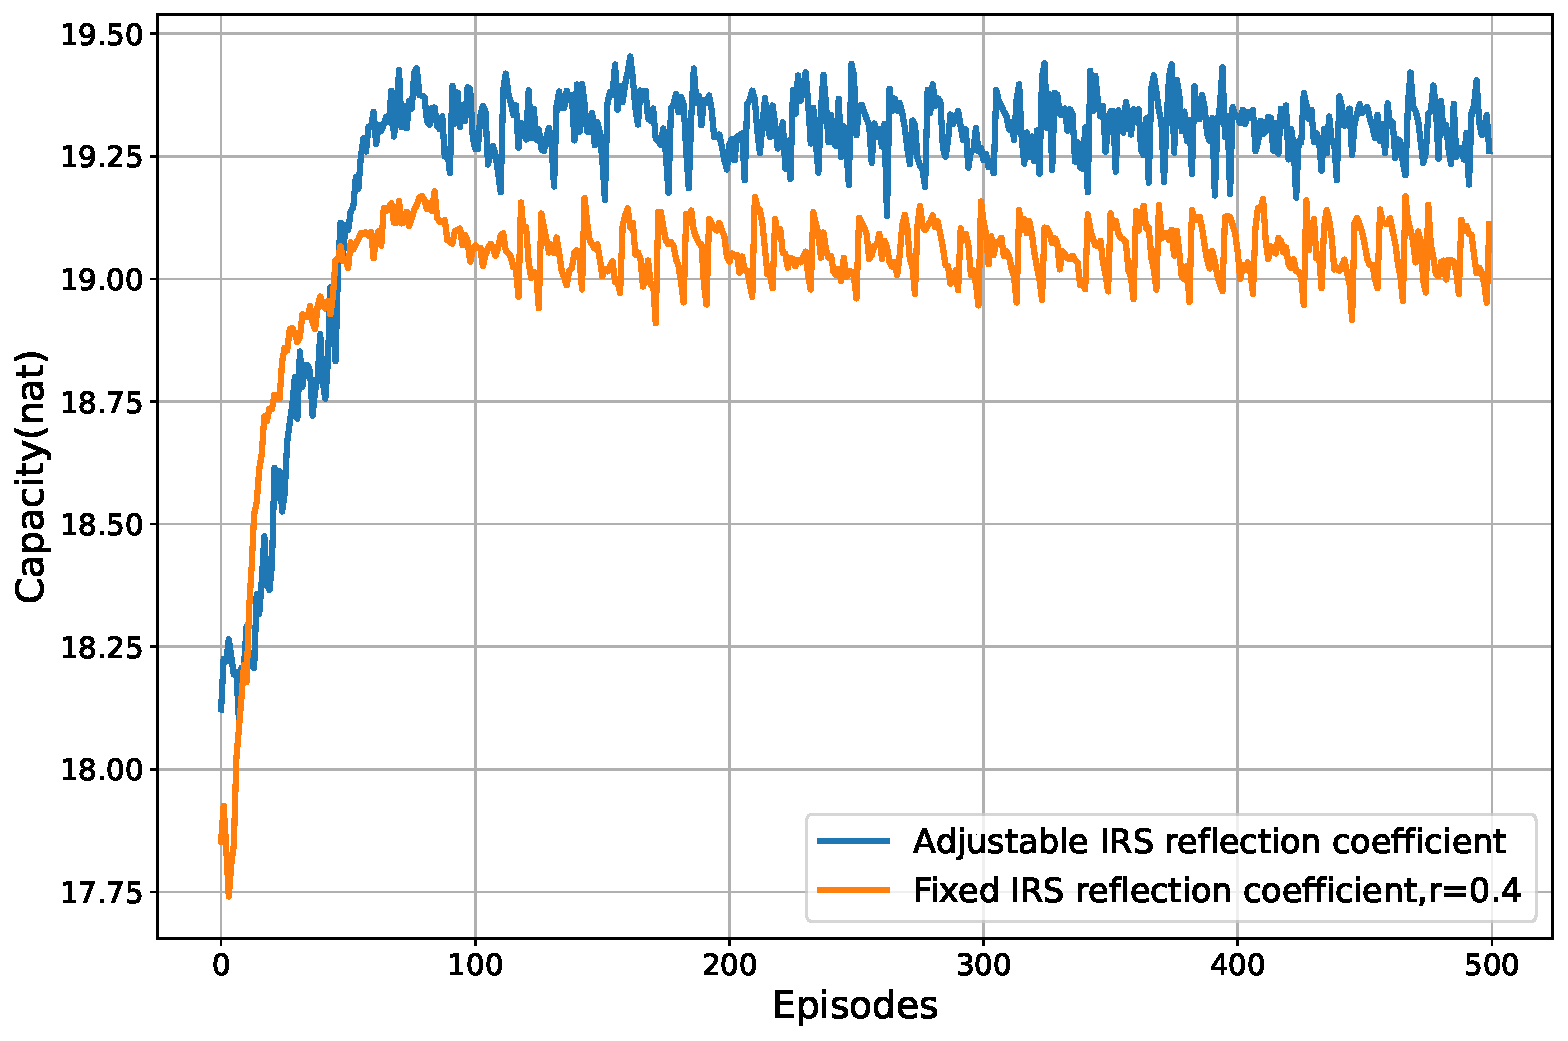
\includegraphics{Capacity with adjustable and fixed reflection.pdf}}
     \caption{Capacity with adjustable and fixed reflection}
     \label{fig:4}
     \end{figure}
     \begin{figure}[htbp]
     \scalebox{0.33}{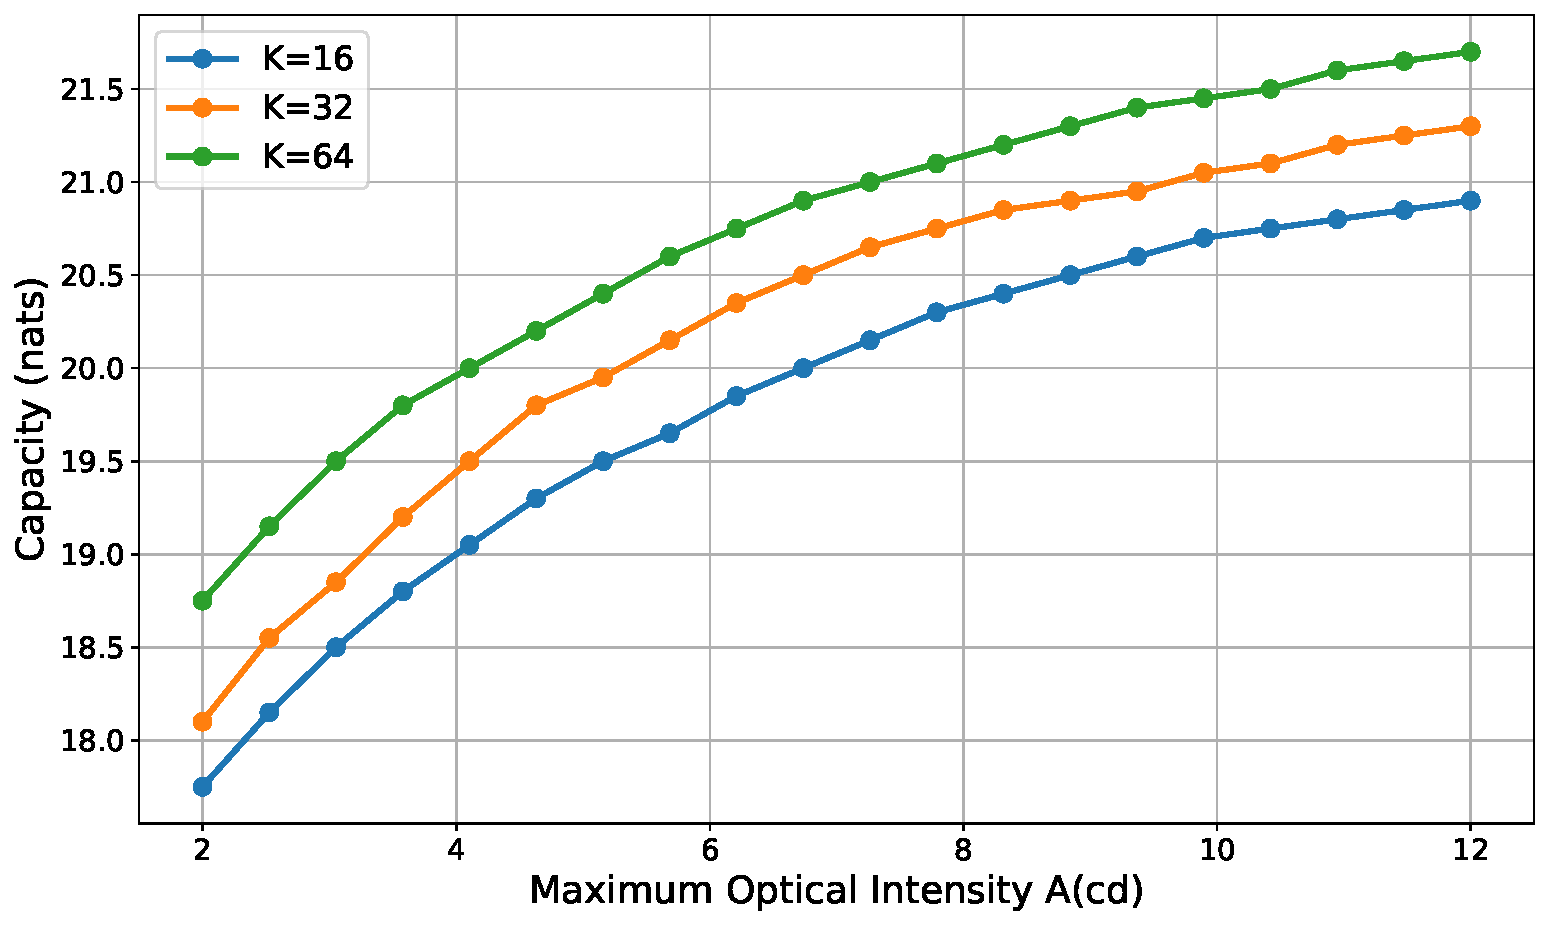
\includegraphics{Capacity with different maximum optical intensity.pdf}}
     \caption{Capacity with different maximum optical intensity.}
     \label{fig:5}
     \end{figure}
     \begin{figure}[htbp]
     \scalebox{0.33}{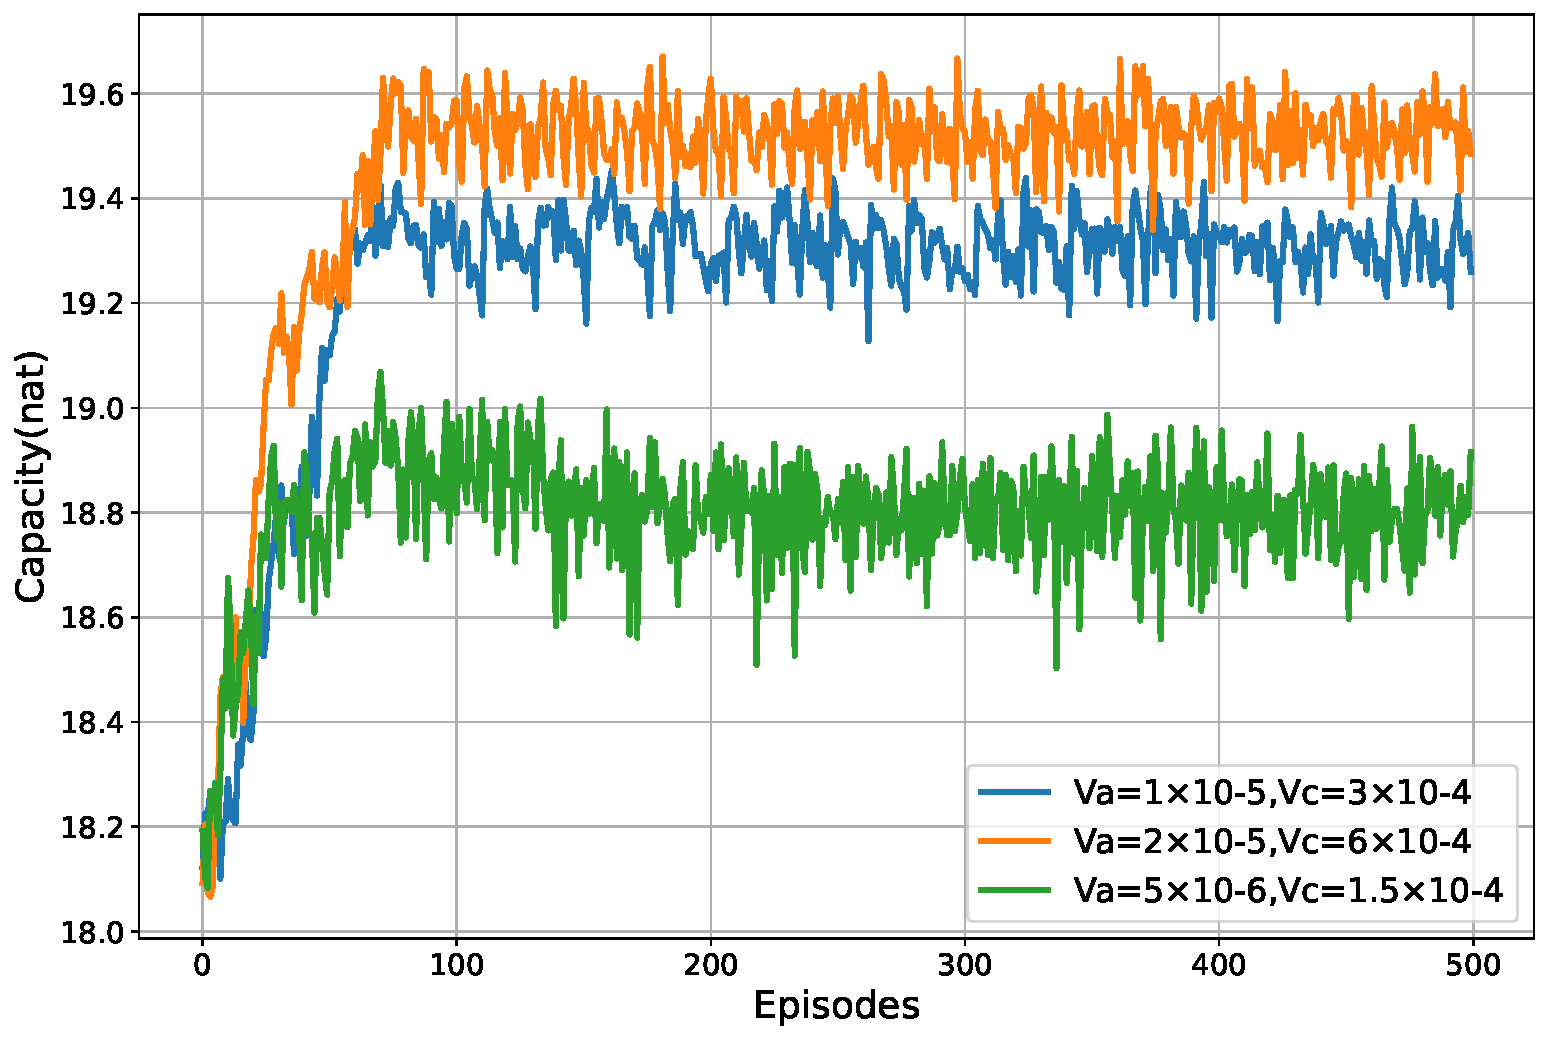
\includegraphics{Capacity with different learning rates（TD3）.pdf}}
     \caption{Capacity with different learning rates（TD3）.}
     \label{fig:6}
     \end{figure}

In Fig.~\ref{fig:4}, we compared the resulting capacity between adjustable and 
fixed IRS reflection coefficients for the same number of thirty-six IRS elements.
It can be seen that the final capacity of the adjustable IRS reflection 
coefficients/ system is significantly higher than that of the fixed 
IRS reflection coefficient system. But at the same time, due to the 
introduction of adjustable IRS coefficients, the computational complexity 
of the algorithm are also increase, meaning that it are also slow down the 
convergence speed.

Next, We compared the change in capacity with maximum optical intensity 
under different IRS in Fig.~\ref{fig:5}. 
When $K$ is constant, the capacity of the system increases 
significantly as the maximum optical intensity increases.

We also compare the capacity at different learning rates when $K$=36 which 
can be seen from Fig.~\ref{fig:6}. As the learning rate changes, the maximum 
capacity that the system can achieve decreases, and the maximum capacity can 
only be reached when the actor network learning rate is equal to $1 \times {10^{ - 5}}$. 
At the same time, as the learning rate decreases, the convergence speed slows down, 
and on the contrary, the system becomes unstable.
     \begin{figure}[htbp]
     \scalebox{0.33}{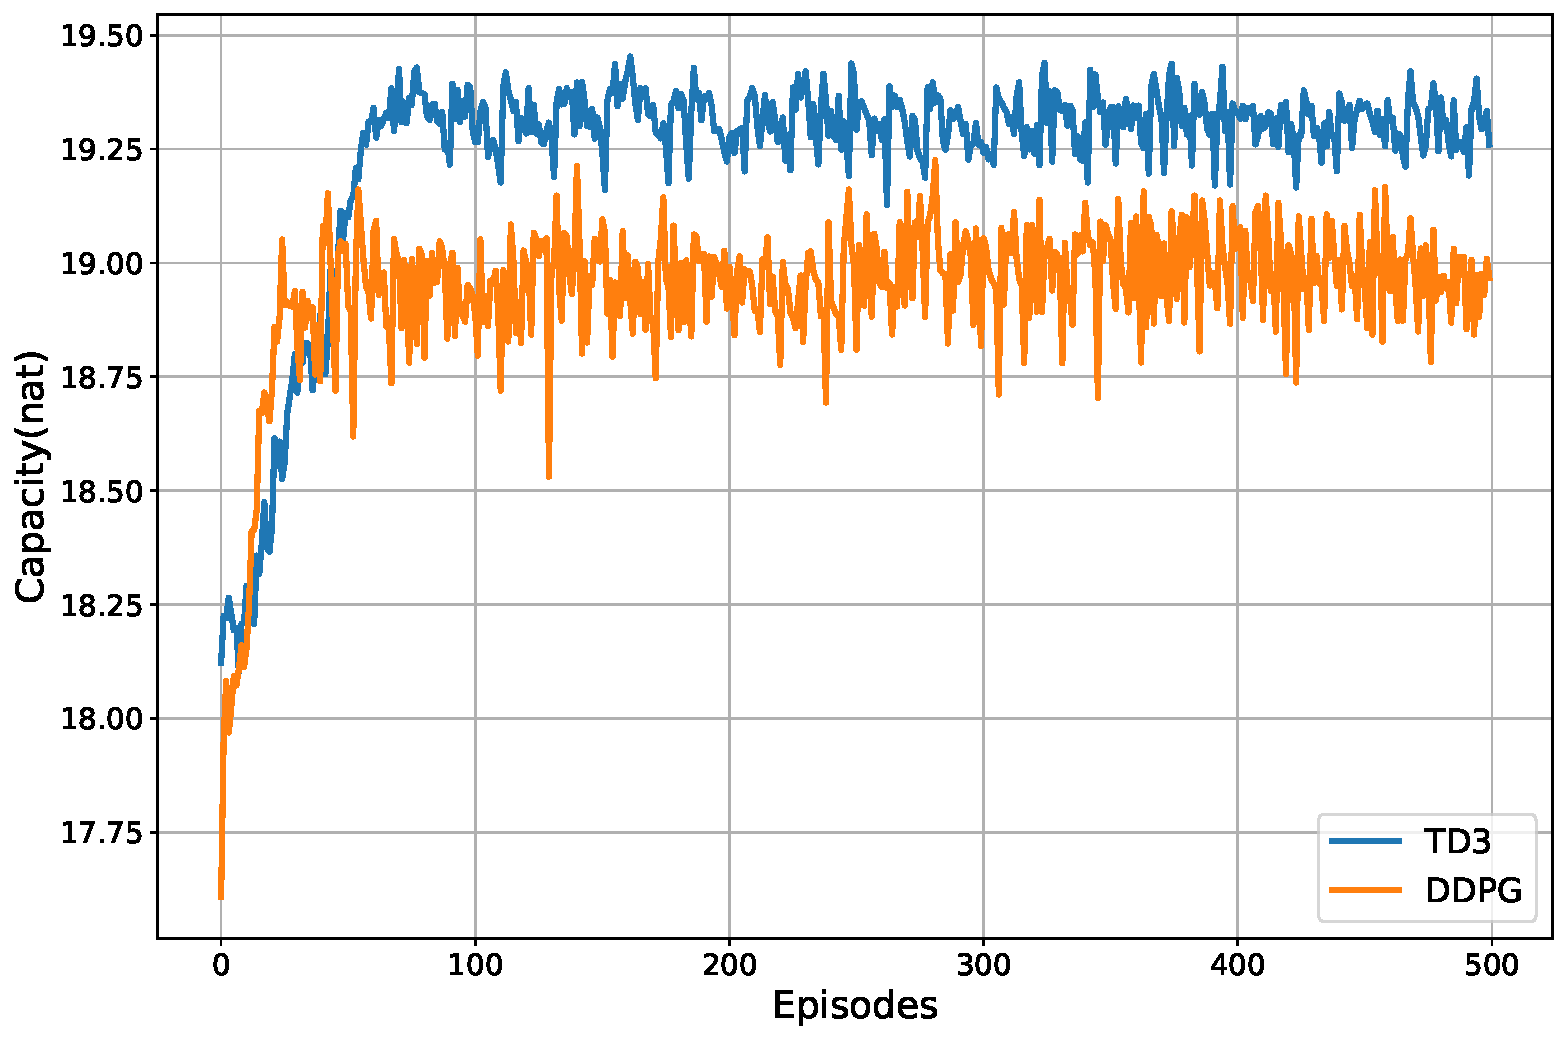
\includegraphics{Comparison of the capacity of DDPG and TD3.pdf}}
     \caption{Comparison of the capacity of DDPG and TD3.}
     \label{fig:7}
     \end{figure}

Finally, in Fig.~\ref{fig:7}, we compared the  different performance between the 
deep deterministic policy gradient (DDPG) algorithm 
and the TD3 algorithm in the same simulation environment. Since TD3 has an 
additional critic network than DDPG, the $Q$ value of each critic network update 
is taken as the smaller of the two critic networks. Therefore, the TD3 algorithm 
can reduce the overestimation bias in DDPG and make the final algorithm results 
more stable and higher.
\section{CONCLUSIONS}
In this paper, we jointly optimized the pairing matrix and reflection coefficient 
vector of IRS elements and the power allocation vector of LED based on the TD3 
algorithm to maximize the capacity of the system. By describing the optimization 
problem as MDP, the computational complexity of the optimization problem 
can be significantly reduced. Finally, we also compare the performance of the 
respective algorithms of TD3 and DDPG. The results show that the TD3 algorithm 
successfully converges and calculates the final size of the maximum capacity, 
and also proves that TD3 has better performance than DDPG in maximizing capacity.

\begin{thebibliography}{00}
\bibitem{1} R. W. Heath, N. González-Prelcic, S. Rangan, W. Roh and A. M. Sayeed, "An Overview of Signal Processing Techniques for Millimeter Wave MIMO Systems," in IEEE Journal of Selected Topics in Signal Processing, vol. 10, no. 3, pp. 436-453, April 2016, doi: 10.1109/JSTSP.2016.2523924.
%\bibitem{2} F. R. Gfeller and U. Bapst, "Wireless in-house data communication via diffuse infrared radiation," in Proceedings of the IEEE, vol. 67, no. 11, pp. 1474-1486, Nov. 1979, doi: 10.1109/PROC.1979.11508.
\bibitem{3}	T. Komine and M. Nakagawa, "Fundamental analysis for visible-light communication system using LED lights," in IEEE Transactions on Consumer Electronics, vol. 50, no. 1, pp. 100-107, Feb. 2004, doi: 10.1109/TCE.2004.1277847. 
\bibitem{4}	M. Obeed, A. M. Salhab, M. -S. Alouini and S. A. Zummo, "On Optimizing VLC Networks for Downlink Multi-User Transmission: A Survey," in IEEE Communications Surveys \& Tutorials, vol. 21, no. 3, pp. 2947-2976, thirdquarter 2019, doi: 10.1109/COMST.2019.2906225.
\bibitem{5} K. -H. Park, Y. -C. Ko and M. -S. Alouini, "On the power and offset allocation for rate adaptation of spatial multiplexing in optical wireless MIMO channels," 2011 7th International Wireless Communications and Mobile Computing Conference, Istanbul, Turkey, 2011, pp. 141-146, doi: 10.1109/IWCMC.2011.5982521.
\bibitem{6}	C. Chen, W. -D. Zhong, D. Wu and Z. Ghassemlooy, "Wide-FOV and High-Gain Imaging Angle Diversity Receiver for Indoor SDM-VLC Systems," in IEEE Photonics Technology Letters, vol. 28, no. 19, pp. 2078-2081, 1 Oct.1, 2016, doi: 10.1109/LPT.2016.2584185.
\bibitem{7}	S. Sun, T. Wang, F. Yang, J. Song and Z. Han, "Intelligent Reflecting Surface-Aided Visible Light Communications: Potentials and Challenges," in IEEE Vehicular Technology Magazine, vol. 17, no. 1, pp. 47-56, March 2022, doi: 10.1109/MVT.2021.3127869.
%\bibitem{8}	A. Nuwanpriya, S. -W. Ho and C. S. Chen, "Indoor MIMO Visible Light Communications: Novel Angle Diversity Receivers for Mobile Users," in IEEE Journal on Selected Areas in Communications, vol. 33, no. 9, pp. 1780-1792, Sept. 2015, doi: 10.1109/JSAC.2015.2432514.
\bibitem{9}	Y. Zhai, H. Chi, J. Tong and J. Xi, "Capacity Maximized Linear Precoder Design for Spatial-Multiplexing MIMO VLC Systems," in IEEE Access, vol. 8, pp. 63901-63909, 2020, doi: 10.1109/ACCESS.2020.2983517.
%\bibitem{10}	B. G. Guzman, M. M. Cespedes, V. P. G. Jimenez, A. G. Armada and M. Brandt-Pearce, "Optimal Mirror Placement to Minimize the Outage Area in Visible Light Communication," GLOBECOM 2023 - 2023 IEEE Global Communications Conference, Kuala Lumpur, Malaysia, 2023, pp. 4698-4703, doi: 10.1109/GLOBECOM54140.2023.10436718.
%\bibitem{11}	S. Sun, F. Yang, J. Song and R. Zhang, "Intelligent Reflecting Surface for MIMO VLC: Joint Design of Surface Configuration and Transceiver Signal Processing," in IEEE Transactions on Wireless Communications, vol. 22, no. 9, pp. 5785-5799, Sept. 2023, doi: 10.1109/TWC.2023.3236811. 
\bibitem{12}	N. Ullah, R. Zhao, and L. Huang, “Recent Advancement in Optical Metasurface: Fundament to Application,” Micromachines, vol. 13, no. 7, p. 1025, Jun. 2022.
\bibitem{13}	T. He, T. Liu, S. Xiao, Z WEI, Z. WANG, L. Zhou AND X Cheng, "Perfect Anomalous Reflectors at Optical Frequencies," in Science Advances, vol. 8, no. 9,2022.
\bibitem{14}	S. Abdollahramezani, O. Hemmatyar, M. Taghinejad, et al. "Electrically driven reprogrammable phase-change metasurface reaching 80\% efficiency," in Nature Communications, vol. 13, 1696, 2022.
\bibitem{15}	B. Chen, X. Wang, W. Li, Chun Li and Z. Wang, et al, "Electrically Addressable Integrated Intelligent Terahertz Metasurface, " in Science Advances vol. 8, no. 41, 2022.
\bibitem{16}	A. A. Hammadi, L. Bariah, S. Muhaidat, M. Al-Qutayri, P. C. Sofotasios and M. Debbah, "Deep Q-Learning-Based Resource Management in IRS-Assisted VLC Systems," in IEEE Transactions on Machine Learning in Communications and Networking, vol. 2, pp. 34-48, 2024, doi: 10.1109/TMLCN.2023.3328501. 
\bibitem{17}	S. Sun, W. Mei, F. Yang, N. An, J. Song and R. Zhang, "Optical Intelligent Reflecting Surface Assisted MIMO VLC: Channel Modeling and Capacity Characterization," in IEEE Transactions on Wireless Communications, vol. 23, no. 3, pp. 2125-2139, March 2024, doi: 10.1109/TWC.2023.3295793.
\bibitem{18}	D. Pereira-Ruisánchez, Ó. Fresnedo, D. Pérez-Adán and L. Castedo, "Deep Contextual Bandit and Reinforcement Learning for IRS-Assisted MU-MIMO Systems," in IEEE Transactions on Vehicular Technology, vol. 72, no. 7, pp. 9099-9114, July 2023, doi: 10.1109/TVT.2023.3249353.
\end{thebibliography}
\end{document}